%%indicações matemática
\documentclass[a4paper,12pt]{article}
\usepackage[brazil]{babel}
\usepackage{fancyhdr}  % Pacote para editar cabeçalhos
\usepackage{graphicx}   % Pacote para inserir imagens
\usepackage{amsmath, amssymb}
\usepackage{geometry}
\usepackage{multicol}
\geometry{left=1cm,right=1cm,top=1cm,bottom=1cm}
\usepackage{enumitem}	
\usepackage{titlesec}
\titleformat{\section}{\footnotesize\bfseries}{\thesection}{1em}{}


% Remove a linha preta do cabeçalho
\renewcommand{\headrulewidth}{0pt}  


\pagestyle{fancy}  % Ativa o estilo de cabeçalho
\fancyhf{} % Limpa cabeçalhos e rodapés

% Adiciona as imagens no cabeçalho, ajustando a escala conforme necessário
\fancyhead[L]{\hspace{7cm}\raisebox{-3cm}{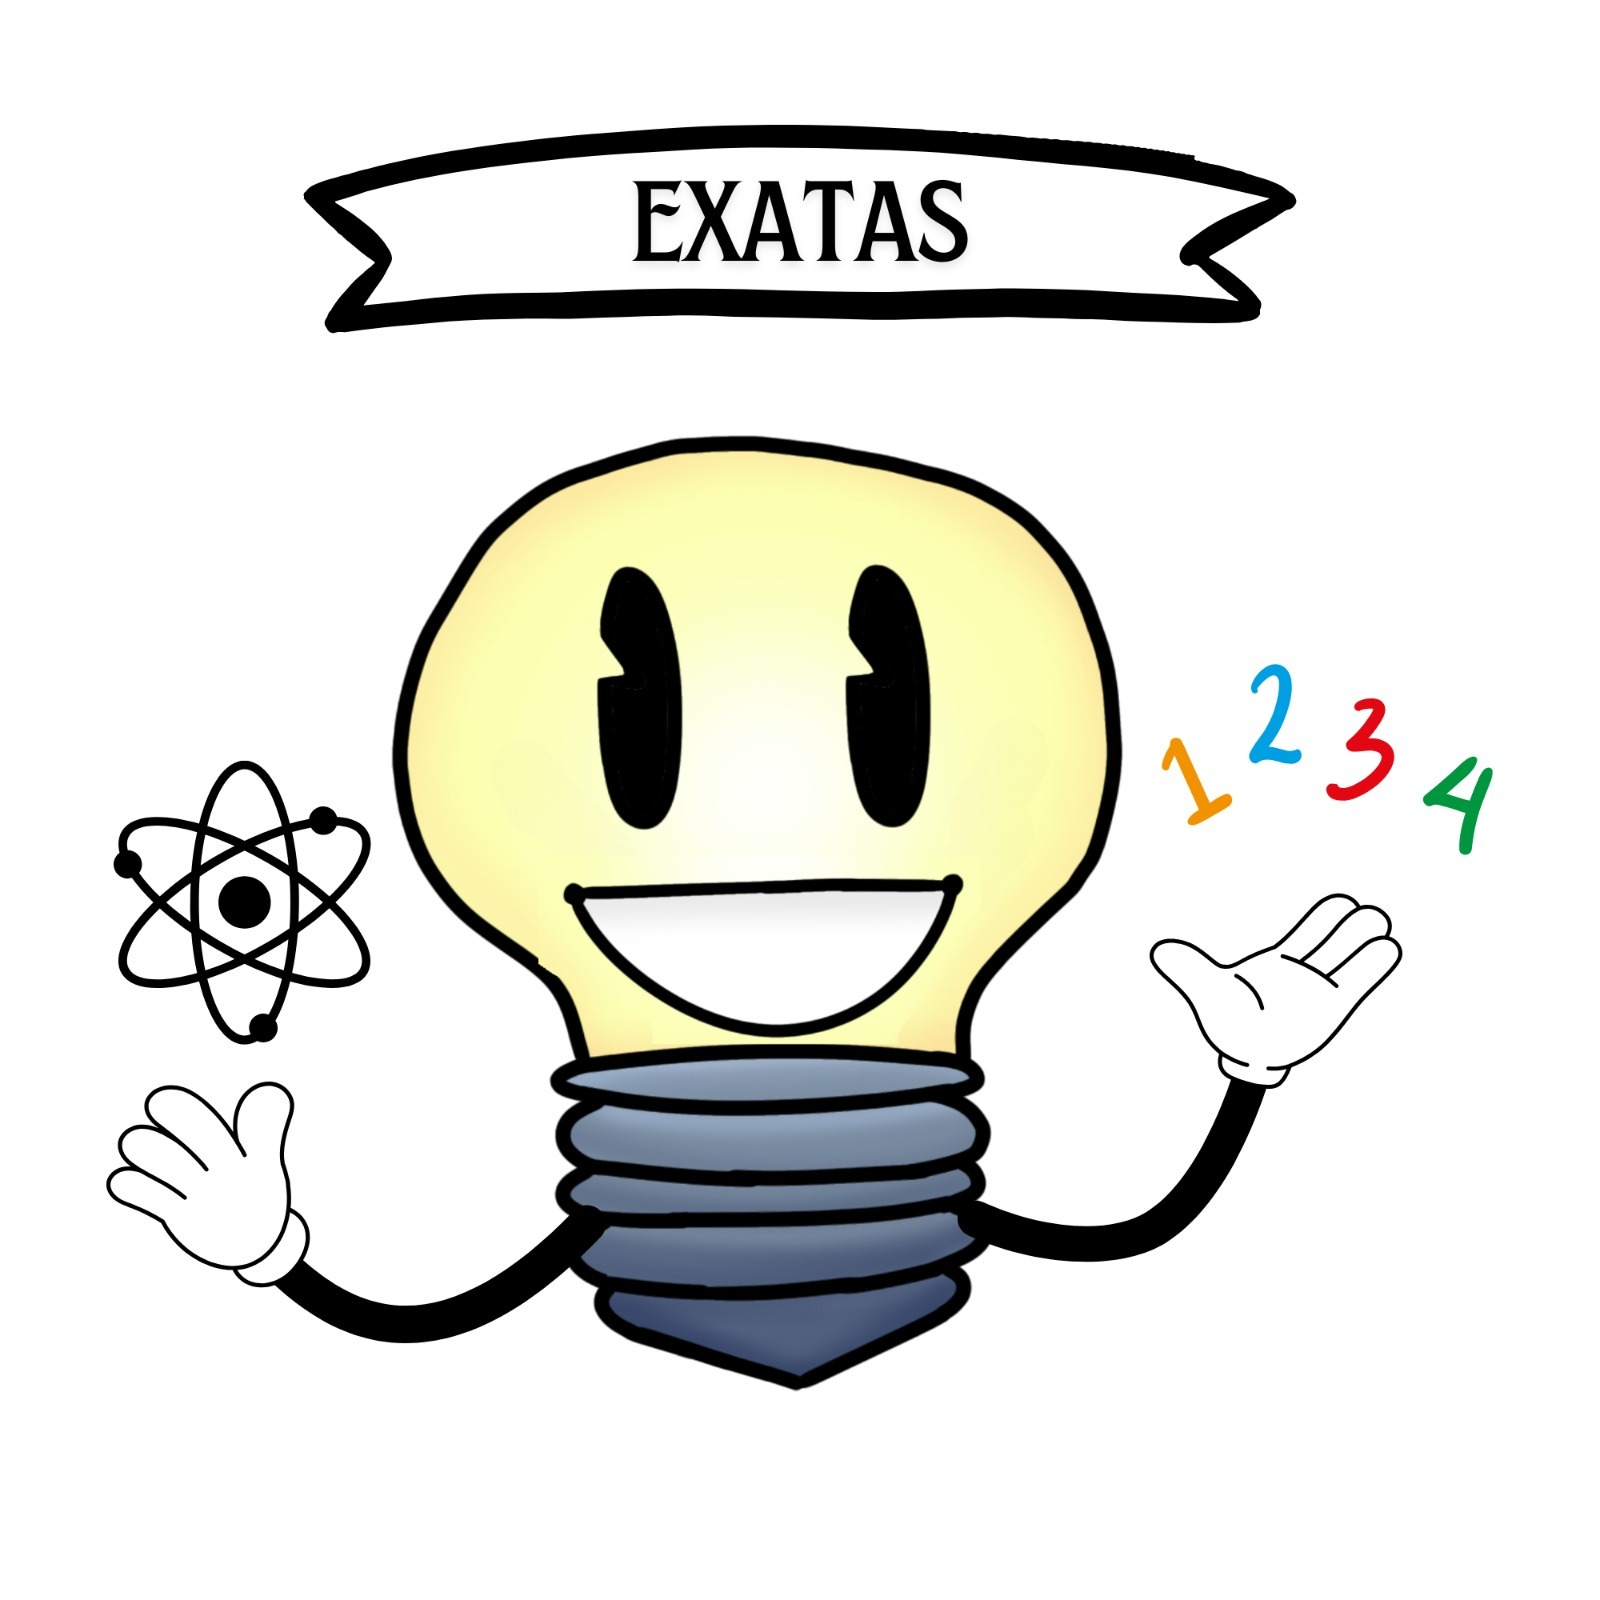
\includegraphics[width=3cm]{exata.jpg}}}  % Esquerda
\fancyhead[R]{\hspace{1cm}\raisebox{-2.5cm}{
\includegraphics[width=4cm]{pei.jpg}}} % Direita

\begin{document}	


\section*{Indicações para estudos}

\begin{enumerate}
	\item \textbf{Canais em Português:}
	\begin{itemize}
		\item Matemática Rio (Rafael Procopio) - @MatematicaRio – Explicações didáticas e divertidas sobre diversos temas de matemática.
		
		\item	Ferretto Matemática - @professorferretto
		– Focado no ensino médio, ENEM e vestibulares.
		
		\item Matemática com Rafa Jesus - Tá Lembrando? - @rafajesus\_talembrando
		– Aborda desde conteúdos básicos até os mais avançados.
		
		\item 	Vestibulandia - @nerckie
		– Muito útil para quem quer se aprofundar em matemática para concursos e vestibulares.
		
		\item	Khan Academy Brasil - @khanacademyportugue – Explicações detalhadas com vídeos bem organizados.
		
		\item	Dicasdemat Sandro Curió -
		@sandrocuriodicasdemat
		– Explicações curtas e diretas sobre diversos tópicos.
		
		\item Gis com Giz Matemática - @Giscomgiz – Explicações curtas e diretas sobre diversos tópicos.
		
		\item Toda a Matemática
		- @todaamatematica - A matemática das suas origens às últimas pesquisas.
		
		\item Professora Angela Matemática
		- @professoraangelamatematica
		- é possível aprender matemática e também gostar dela.
		
		\item Professor Dr. Rafael Bastos Mr. Bean da Matemática
		- @mrbeandamatematica
		- Com o Mr Bean da Matemática o aprendizado se torna muito mais fácil. 
		
		\item Estude Matemática
		- @estudematematica - Conteúdo para entusiastas da Matemática...
		
		\item Universo Narrado
		- @UniversoNarrado
		- Narrativas que buscam explorar a beleza do universo por meio da ciência e da literatura.
		
		\item Prof. MURAKAMI - MATEMÁTICA RAPIDOLA
		- @Murakami.
		- Aprenda em pouco tempo e de forma simples, temas em muitos casos considerados difíceis e tenha uma excelente preparação para as suas provas.
		
	\end{itemize}
	
	\item \textbf{Canais em Inglês:}
	
	\begin{itemize}
		\item 	3Blue1Brown - @3blue1brown– Explica matemática de forma visual e intuitiva.
		
		\item 	Khan Academy - @khanacademy – Um dos maiores canais educacionais, cobrindo desde matemática básica até cálculo avançado.
		
		\item 	Numberphile  - @numberphile – Explora conceitos matemáticos de forma curiosa e divertida.
		
		\item 	PatrickJMT - @patrickjmt – Explica matemática de forma clara e objetiva.
		
		\item 	Mathologer  - @Mathologer – Aborda matemática avançada com uma pegada histórica e visual.
		
		\item 	Eddie Woo - @misterwootube – Ensina matemática de maneira acessível e envolvente.
		
		
		
	\end{itemize}
	
	\item \textbf{Plataformas e Sites Educacionais:}
	\begin{itemize}
		\item 	Khan Academy – Plataforma gratuita com vídeos, exercícios e acompanhamento de progresso.
		
		\item	Brasil Escola – Explicações teóricas, exercícios e materiais de apoio.
		
		\item		Só Matemática – Exercícios, jogos matemáticos e materiais didáticos.
		
		\item 	Descomplica – Plataforma paga com aulas para ensino médio e vestibulares.
		
		\item		Fuvestibular – Material gratuito para vestibulares e Enem.
	\end{itemize}
	
	
	
	
\end{enumerate}


\end{document}